\section{Уменьшение размерности}
Уменьшение размерности и визуализация. 

Обе эти задачи состоят в сжатии выборки: нужно перевести точки из \textit{N-мерного} пространства в \textit{M-мерное} пространство, где $M < N$, причем так, чтобы близкие точки остались близкими. То есть хочется значительно уменьшить число признаков, не сильно потеряв (или даже улучшив) их качество.
\subsection{SVD-разложение}
Пусть $A$ - прямоугольная матрица признаков. Тогда она представима единственным образом в следующем виде:
\begin{equation}
    A = U \Sigma V
\end{equation}

где:

$\Sigma$ -- прямоугольная диагональная матрица с неотрицательными убывающими элементами на диагонали,

$U, V$ -- квадратные унитарные матрицы

Cмысл такой, что преобразование пространства под действием оператора с унитарной матрицей -- сохраняет скалярное произведение, то есть грубо говоря это поворот пространства. 

Существует теорема Эккарта-Янга, которая утверждает, что можно приблизить матрицу $A$ матрицей меньшего ранга $k < n$, причем наилучшая матрица(в плане минимальной нормы разницы матриц) -- будет матрица полученная усечённым \textbf{SVD-разложением}.

\subsubsection*{Усечённое SVD-разложение}
Выберем $k$ -- ранг матрицы, которой будем приближать исходную матрицу $A$, с практической точки зрения это количество признаков, которые мы хотим оставить.

Применим SVD-разложение. 

$$A = U \Sigma V$$

Оставим только $k$ столбцов в $U$ и $k$ строк в $V$, а так же занулим все, кроме $k$ первых чисел на диагонали в $\Sigma$, обрежем ее до размерности $k \cdot k$.

Назовём это $A_{k} = U_{k} \Sigma_{k} V_{k}$. 

Такое приближение матрицы $A$ матрицей ранга $k$ -- оптимально, а матрица $U_{k} \Sigma_{k}$ -- называется \textbf{усечённым SVD-разложением} матрицы $A$ и содержит ровно $k$ столбцов, то есть уменьшилось количество признаков.
В sklearn этот метод лежит в sklearn.decomposition.TruncatedSVD.

\subsection{PCA - метод главных компонент}

Метод \textbf{PCA} заключается в том, чтобы найти в N-мерном пространстве такое K-мерное пространство, что проекция всех точек на него будет как можно более рассеянной (то есть иметь наибольшую дисперсию).

Оказывается, подходит пространство, сумма квадратов расстояния от которого до всех точек минимальна.

Первая компонента (ось) выбирается так, чтобы дисперсия проекции вдоль нее была максимальна.

После этого все точки проецируются вдоль первой компоненты и там таким же способом выбирается вторая компонента и так далее.

Получившиеся $k$ компонент будут образовывать K-мерное пространство, проекция точек на которое будет иметь наибольшую дисперсию.

Оказывается, если применить \textit{TruncatedSVD} к центрированным данным (среднее по каждой координате равно 0), то именно это и получится!

В каком-то смысле PCA - это лучший линейный способ уменьшить размерность пространства.

\begin{center}
    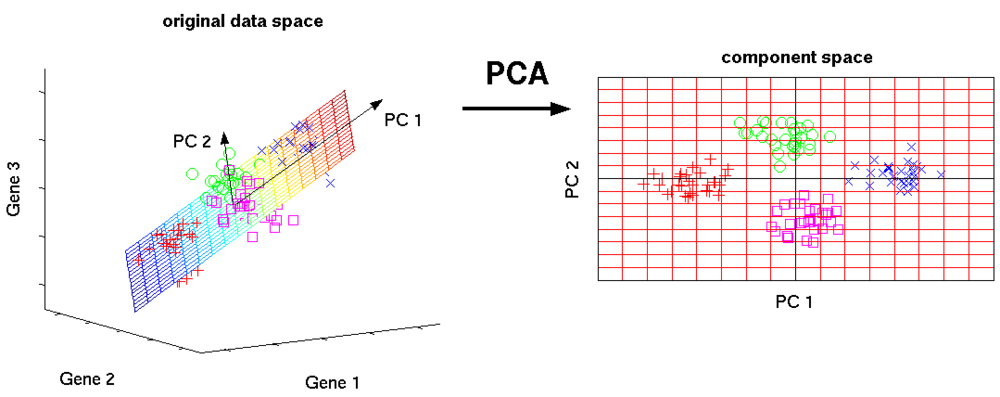
\includegraphics[scale=0.5]{tickets/pictures/pca.png}
\end{center}
\begin{center}
    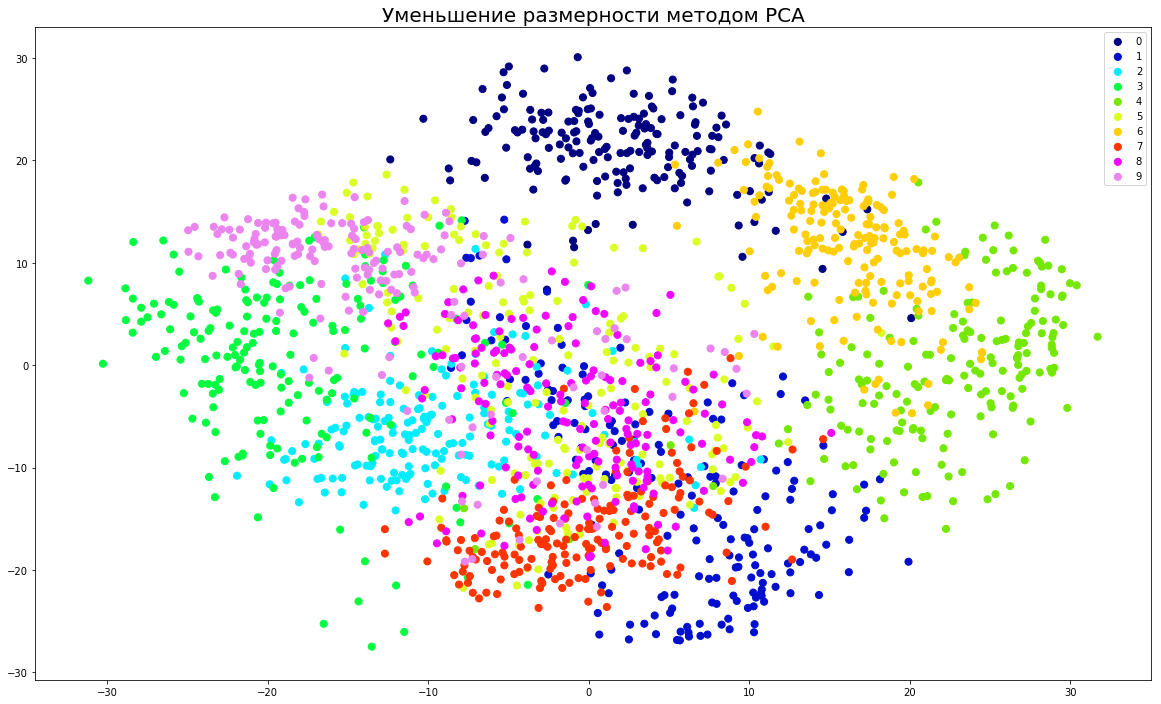
\includegraphics[scale=0.45]{tickets/pictures/pca_sample.png}
\end{center}
\subsubsection*{Плюсы PCA}
\begin{itemize}
    \item считается относительно быстро
    \item детерминированность (зависит от реализации, в sklearn не так)
    \item любая размерность
    \item полученную модель уменьшения размерности можно применять и к новым точкам (нужно просто спроецировать ее на выделенное $k$-мерное пространство)
    \item визуализация при $k = 2$ - это честная проекция на какую-то плоскость, легкая интерпретируемость результатов
    \item при увеличении размерности старые координаты не меняются
    \item отлично подходит для отбора признаков
\end{itemize}

\subsubsection*{Минусы PCA}
\begin{itemize}
    \item алгоритм слишком простой - он линейный
    \item некоторые непохожие точки могут спроецироваться в одну и ту же при $k = 2$
\end{itemize}

\subsection{t-SNE}
Это гораздо более сложный нелинейный алгоритм. Он очень крут для визуализации данных, и работает только с переводом в 2D и 3D.

Внутри там происходит что-то физическое - элементы будто разлетаются, причем чем дальше они друг от друга, тем сильнее они друг друга оттакливают.

\begin{center}
    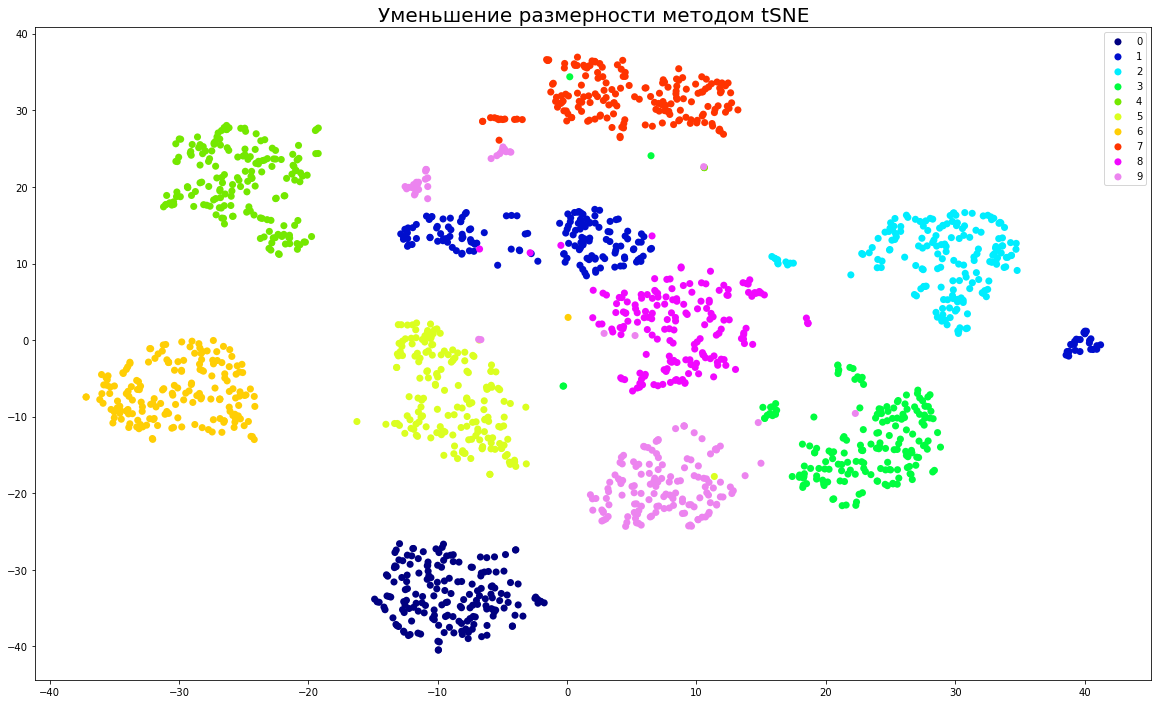
\includegraphics[scale=0.45]{tickets/pictures/tsne_sample.png}
\end{center}

\subsubsection*{Плюсы t-SNE}
\begin{itemize}
    \item отлично визуализирует (2D, 3D) данные
    \item физически разносит разные точки дальше друг от друга
    \item сильно разные точки не могут в конце оказаться рядом
\end{itemize}

\subsubsection*{Недостатки t-SNE}
\begin{itemize}
    \item недетерминированность, результат меняется при каждом запуске
    \item координаты ничего не значат сами по себе
    \item нельзя легко добавить новые данные
    \item долго работает
    \item уменьшает только до 2 и 3 размерности
\end{itemize}